%%%%%%%%%%%%%%%%%%%%%%%%%%%%%%%%%%%%%%%%%
% University Assignment Title Page 
% LaTeX Template
%
% This template has been downloaded from:
% http://www.latextemplates.com
%
% Original author:
% WikiBooks (http://en.wikibooks.org/wiki/LaTeX/Title_Creation)
% 
% Instructions for using this template:
% This title page is presently capable of being compiled as is. This is not 
% useful for including it in another document. To do this, you have two options: 
%
% 1) Copy/paste everything between \begin{document} and \end{document} 
% starting at \begin{titlepage} and paste this into another LaTeX file where you 
% want your title page.
% OR
% 2) Remove everything outside the \begin{titlepage} and \end{titlepage} and 
% move this file to the same directory as the LaTeX file you wish to add it to. 
% Then add %%%%%%%%%%%%%%%%%%%%%%%%%%%%%%%%%%%%%%%%%
% University Assignment Title Page 
% LaTeX Template
%
% This template has been downloaded from:
% http://www.latextemplates.com
%
% Original author:
% WikiBooks (http://en.wikibooks.org/wiki/LaTeX/Title_Creation)
% 
% Instructions for using this template:
% This title page is presently capable of being compiled as is. This is not 
% useful for including it in another document. To do this, you have two options: 
%
% 1) Copy/paste everything between \begin{document} and \end{document} 
% starting at \begin{titlepage} and paste this into another LaTeX file where you 
% want your title page.
% OR
% 2) Remove everything outside the \begin{titlepage} and \end{titlepage} and 
% move this file to the same directory as the LaTeX file you wish to add it to. 
% Then add %%%%%%%%%%%%%%%%%%%%%%%%%%%%%%%%%%%%%%%%%
% University Assignment Title Page 
% LaTeX Template
%
% This template has been downloaded from:
% http://www.latextemplates.com
%
% Original author:
% WikiBooks (http://en.wikibooks.org/wiki/LaTeX/Title_Creation)
% 
% Instructions for using this template:
% This title page is presently capable of being compiled as is. This is not 
% useful for including it in another document. To do this, you have two options: 
%
% 1) Copy/paste everything between \begin{document} and \end{document} 
% starting at \begin{titlepage} and paste this into another LaTeX file where you 
% want your title page.
% OR
% 2) Remove everything outside the \begin{titlepage} and \end{titlepage} and 
% move this file to the same directory as the LaTeX file you wish to add it to. 
% Then add %%%%%%%%%%%%%%%%%%%%%%%%%%%%%%%%%%%%%%%%%
% University Assignment Title Page 
% LaTeX Template
%
% This template has been downloaded from:
% http://www.latextemplates.com
%
% Original author:
% WikiBooks (http://en.wikibooks.org/wiki/LaTeX/Title_Creation)
% 
% Instructions for using this template:
% This title page is presently capable of being compiled as is. This is not 
% useful for including it in another document. To do this, you have two options: 
%
% 1) Copy/paste everything between \begin{document} and \end{document} 
% starting at \begin{titlepage} and paste this into another LaTeX file where you 
% want your title page.
% OR
% 2) Remove everything outside the \begin{titlepage} and \end{titlepage} and 
% move this file to the same directory as the LaTeX file you wish to add it to. 
% Then add \input{./title_page_1.tex} to your LaTeX file where you want your
% title page.
%
%%%%%%%%%%%%%%%%%%%%%%%%%%%%%%%%%%%%%%%%%

%----------------------------------------------------------------------------------------
%	PACKAGES AND OTHER DOCUMENT CONFIGURATIONS
%----------------------------------------------------------------------------------------

\documentclass[12pt]{article}

\begin{document}

\begin{titlepage}

\newcommand{\HRule}{\rule{\linewidth}{0.5mm}} % Defines a new command for the horizontal lines, change thickness here

\center % Center everything on the page
 
%----------------------------------------------------------------------------------------
%	HEADING SECTIONS
%----------------------------------------------------------------------------------------

\textsc{\LARGE}\\[1.5cm] % Name of your university/college
\textsc{\Large Computer System Engineering}\\[0.5cm] % Major heading such as course name
\textsc{\large Design Project 1 Report}\\[0.5cm] % Minor heading such as course title

%----------------------------------------------------------------------------------------
%	TITLE SECTION
%----------------------------------------------------------------------------------------

\HRule \\[0.4cm]
{ \huge \bfseries Create a Versioning File System}\\[0.4cm] % Title of your document
\HRule \\[1.5cm]
 
%----------------------------------------------------------------------------------------
%	AUTHOR SECTION
%----------------------------------------------------------------------------------------

% If you don't want a supervisor, uncomment the two lines below and remove the section above
\Large \emph{Author:}\\
Bo Song  \textsc{11302010003}\\% Your name
YiTing Cheng  \textsc{11302010050}\\% Your name
YuWei Zhou  \textsc{11302010067}\\[3cm]% Your name

%----------------------------------------------------------------------------------------
%	DATE SECTION
%----------------------------------------------------------------------------------------

{\large \today}\\[3cm] % Date, change the \today to a set date if you want to be precise

%----------------------------------------------------------------------------------------
%	LOGO SECTION
%----------------------------------------------------------------------------------------

%\includegraphics{Logo}\\[1cm] % Include a department/university logo - this will require the graphicx package
 
%----------------------------------------------------------------------------------------

\vfill % Fill the rest of the page with whitespace

\end{titlepage}
\end{document} to your LaTeX file where you want your
% title page.
%
%%%%%%%%%%%%%%%%%%%%%%%%%%%%%%%%%%%%%%%%%

%----------------------------------------------------------------------------------------
%	PACKAGES AND OTHER DOCUMENT CONFIGURATIONS
%----------------------------------------------------------------------------------------

\documentclass[12pt]{article}

\begin{document}

\begin{titlepage}

\newcommand{\HRule}{\rule{\linewidth}{0.5mm}} % Defines a new command for the horizontal lines, change thickness here

\center % Center everything on the page
 
%----------------------------------------------------------------------------------------
%	HEADING SECTIONS
%----------------------------------------------------------------------------------------

\textsc{\LARGE}\\[1.5cm] % Name of your university/college
\textsc{\Large Computer System Engineering}\\[0.5cm] % Major heading such as course name
\textsc{\large Design Project 1 Report}\\[0.5cm] % Minor heading such as course title

%----------------------------------------------------------------------------------------
%	TITLE SECTION
%----------------------------------------------------------------------------------------

\HRule \\[0.4cm]
{ \huge \bfseries Create a Versioning File System}\\[0.4cm] % Title of your document
\HRule \\[1.5cm]
 
%----------------------------------------------------------------------------------------
%	AUTHOR SECTION
%----------------------------------------------------------------------------------------

% If you don't want a supervisor, uncomment the two lines below and remove the section above
\Large \emph{Author:}\\
Bo Song  \textsc{11302010003}\\% Your name
YiTing Cheng  \textsc{11302010050}\\% Your name
YuWei Zhou  \textsc{11302010067}\\[3cm]% Your name

%----------------------------------------------------------------------------------------
%	DATE SECTION
%----------------------------------------------------------------------------------------

{\large \today}\\[3cm] % Date, change the \today to a set date if you want to be precise

%----------------------------------------------------------------------------------------
%	LOGO SECTION
%----------------------------------------------------------------------------------------

%\includegraphics{Logo}\\[1cm] % Include a department/university logo - this will require the graphicx package
 
%----------------------------------------------------------------------------------------

\vfill % Fill the rest of the page with whitespace

\end{titlepage}
\end{document} to your LaTeX file where you want your
% title page.
%
%%%%%%%%%%%%%%%%%%%%%%%%%%%%%%%%%%%%%%%%%

%----------------------------------------------------------------------------------------
%	PACKAGES AND OTHER DOCUMENT CONFIGURATIONS
%----------------------------------------------------------------------------------------

\documentclass[12pt]{article}

\begin{document}

\begin{titlepage}

\newcommand{\HRule}{\rule{\linewidth}{0.5mm}} % Defines a new command for the horizontal lines, change thickness here

\center % Center everything on the page
 
%----------------------------------------------------------------------------------------
%	HEADING SECTIONS
%----------------------------------------------------------------------------------------

\textsc{\LARGE}\\[1.5cm] % Name of your university/college
\textsc{\Large Computer System Engineering}\\[0.5cm] % Major heading such as course name
\textsc{\large Design Project 1 Report}\\[0.5cm] % Minor heading such as course title

%----------------------------------------------------------------------------------------
%	TITLE SECTION
%----------------------------------------------------------------------------------------

\HRule \\[0.4cm]
{ \huge \bfseries Create a Versioning File System}\\[0.4cm] % Title of your document
\HRule \\[1.5cm]
 
%----------------------------------------------------------------------------------------
%	AUTHOR SECTION
%----------------------------------------------------------------------------------------

% If you don't want a supervisor, uncomment the two lines below and remove the section above
\Large \emph{Author:}\\
Bo Song  \textsc{11302010003}\\% Your name
YiTing Cheng  \textsc{11302010050}\\% Your name
YuWei Zhou  \textsc{11302010067}\\[3cm]% Your name

%----------------------------------------------------------------------------------------
%	DATE SECTION
%----------------------------------------------------------------------------------------

{\large \today}\\[3cm] % Date, change the \today to a set date if you want to be precise

%----------------------------------------------------------------------------------------
%	LOGO SECTION
%----------------------------------------------------------------------------------------

%\includegraphics{Logo}\\[1cm] % Include a department/university logo - this will require the graphicx package
 
%----------------------------------------------------------------------------------------

\vfill % Fill the rest of the page with whitespace

\end{titlepage}
\end{document} to your LaTeX file where you want your
% title page.
%
%%%%%%%%%%%%%%%%%%%%%%%%%%%%%%%%%%%%%%%%%
\documentclass[12pt]{article}
\usepackage{geometry}                		% See geometry.pdf to learn the layout options. There are lots.
\geometry{letterpaper}                   		% ... or a4paper or a5paper or ... 
%\geometry{landscape}                		% Activate for for rotated page geometry
%\usepackage[parfill]{parskip}    		% Activate to begin paragraphs with an empty line rather than an indent
\usepackage{graphicx}				% Use pdf, png, jpg, or eps� with pdflatex; use eps in DVI mode
								% TeX will automatically convert eps --> pdf in pdflatex		
\usepackage{amssymb}
\setlength{\parindent}{0pt}

%----------------------------------------------------------------------------------------
%	PACKAGES AND OTHER DOCUMENT CONFIGURATIONS
%----------------------------------------------------------------------------------------


\begin{document}

\begin{titlepage}

\newcommand{\HRule}{\rule{\linewidth}{0.5mm}} % Defines a new command for the horizontal lines, change thickness here

\center % Center everything on the page
 
%----------------------------------------------------------------------------------------
%	HEADING SECTIONS
%----------------------------------------------------------------------------------------

\textsc{\LARGE}\\[1.5cm] % Name of your university/college
\textsc{\Large Computer System Engineering}\\[0.5cm] % Major heading such as course name
\textsc{\large Design Project 1 Report}\\[0.5cm] % Minor heading such as course title

%----------------------------------------------------------------------------------------
%	TITLE SECTION
%----------------------------------------------------------------------------------------

\HRule \\[0.4cm]
{ \huge \bfseries Create a Versioning File System}\\[0.4cm] % Title of your document
\HRule \\[1.5cm]
 
%----------------------------------------------------------------------------------------
%	AUTHOR SECTION
%----------------------------------------------------------------------------------------

% If you don't want a supervisor, uncomment the two lines below and remove the section above
\Large \emph{Author:}\\
Bo Song  \textsc{11302010003}\\% Your name
YiTing Cheng  \textsc{11302010050}\\% Your name
YuWei Zhou  \textsc{11302010067}\\[3cm]% Your name

%----------------------------------------------------------------------------------------
%	DATE SECTION
%----------------------------------------------------------------------------------------

{\large \today}\\[3cm] % Date, change the \today to a set date if you want to be precise

%----------------------------------------------------------------------------------------
%	LOGO SECTION
%----------------------------------------------------------------------------------------

%\includegraphics{Logo}\\[1cm] % Include a department/university logo - this will require the graphicx package
 
%----------------------------------------------------------------------------------------

\vfill % Fill the rest of the page with whitespace

\end{titlepage}

\section*{1~~~~Introduction}The goal of this design project is to create a versioning file system. The versioning or continuous snapshotting file system is defined to store all versions of each file over time. When user modifies a file or  a directory, the versioning file system create a new version after closing the file or directory and store the old version which can be only read by users. \\[1em]To implement this system, The whole design will solve two major problem: how to maintain the old version and how to manipulate them, as well as achieving low access time and better space utilization under common use cases.
\section*{2~~~~Design Description}
The versioning file system(VFS) represents different versions of a file or directory as different inodes which is based on the inodes in Unix file system. Therefore, we need add extra fields to origin inode data structure. Then, a new layout and management is required to maintain the huge number of inodes and data blocks. Finally, some interfaces is adopted to let users manipulate different versions easily.
\section*{2.1~~~~Data Structure}
\section*{2.1.1~~~~On-disk Structure}
\begin{figure}[!ht]
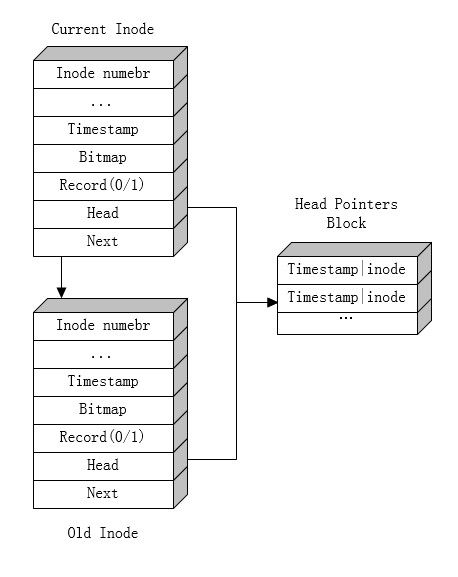
\includegraphics{inode3.png}
\caption{Inode Structure}
\end{figure}
In Unix file system, we treat file and directory as inode on the disk. Similarly, VFS also use inode and there are several fields are added to it as mentioned below(Figure 1). 
\paragraph{Timestamp}When a new version is created, a unsigned integer is recorded, representing the number of seconds passed since a epoch which is predefined in the system. If the unsigned integer is 32 bit, the timestamp allows the system to represent about 132 years after the epoch(typically 1970.1.1) which is enough to current system, and it is easy to extend to 64 bit when we need to represent more time. 
\paragraph{Bitmap}The system embeds bitmaps in inodes and indirect blocks that allow system to record which blocks have had a copy-on-write performed which will discuss in memory management section. A bit of value 0 indicates that a new block needs to be allocated on the next write and bit value 1 indicates that a new allocation of this block has been performed. The size of Bitmap is mainly the overhead of extra fields but we think it worth costing it to optimize performance for its three uses mentioned below.
\paragraph{Next}A pointer to the next old version of an inode. Through this field, we can search a specific version of an inode like an linked list, and the current version inode is the head of linked list. Since the performance of it may not so considerable, a optimized structure will discuss in layout section.
\paragraph{Record}When a user want excludes a file or directory from versioning, an extra bit is employed to indicate it. a bit of value 0 is versioning which is default, and one is not versioning. When the system wants to create a new version, it will first exam this bit and decide whether to do subsequent things.
\paragraph{Head Pointer}A pointer to a block containing addresses of the head of sublists of inodes discussed in layout section. \\[1em]
Since the size of inode  is fixed(typically 2K in fast file system), the number of indirect block pointer fields will decrease after adding new fields and it will result in reduced max file size under approximately 10\% which is acceptable.\\[1em]
Although Record and Head Pointer field is only used in current version inode and waste some space in old versions, the old version is read only and inode is fixed size. Consequently, it is meaningless to free these fields in the old version inode.
\section*{2.2.2~~~~In-memory Structure}

\section*{2.2~~~~Memory Management}
\section*{2.2.1~~~~Copy-on-write}
\begin{figure}[!ht]
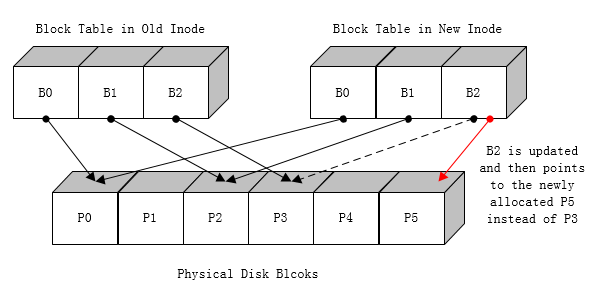
\includegraphics{cow2.png}
\caption{Copy-On-Write Process}
\end{figure}
When a new version is created, it is too waste to copy all the block in the old version. So copy-on-write(abbreviated COW) is adopted to implement multiple versions of data compactly. The system needs to create a new physical version of a file only when data changes. Frequently, physical versions have much data in common. The COW allows versions to share a single copy of file system blocks for common data and have their own copy of data that have changed(Figure 2). As a result, it extremely improves the memory utilization in the system.\\[1em]How COW works is showed in the following steps:
\begin{enumerate}
\item When users open a file or directory, a new inode is duplicated with different inode number and same block references.
\item When users have modified something, the system will allocate new blocks to store modified blocks. The block reference in the new inode will point to the new allocated block and the old one remains unchanged, at the same time, the bitmap in the new inode will also update. 
\item When users finally closed the file, the system check whether the bitmap is all zero. If it is, it means nothing changes and the new inode will free. Otherwise, a new version of inode is finished.
\end{enumerate}
\section*{2.2.2~~~~Garbage Collection} 
When the disk is almost full(A predefined constant such as 90\%), the system also support garbage collection by repeatedly scanning inode table and freeing the oldest inode sublist(discussed in layout section) of each current inode till the space decreased to another predefined constant such as 80\%.
\section*{2.3~~~~Layout}
The problem that the length of a linked inodes list may be very long will cost more time to find a specific old version. Hence, a optimized layout is introduced to solve this problem.
\section*{2.3.1~~~~B-tree Layout}
\section*{2.3.2~~~~ Abandoned Sublists-only Layout}
\begin{figure}[!ht]
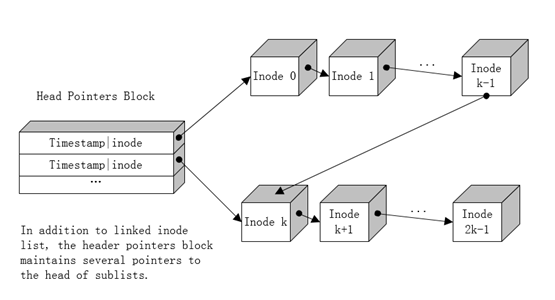
\includegraphics{linkedlist.png}
\caption{Sublists-only Layout}
\end{figure}
When the length of linked inode list exceeds a predefined number k, the system divides it into small sublists. The head of each sublist which contains the address of first inode in the sublist and its timestamp is recorded in a block mentioned in data structure section(Figure 3). When the user find a version of file with given timestamp, the system use the timestamp as a key and search the sublist containing that inode efficiently with a function.
\section*{2.4~~~~Interfaces and Manipulating Old Versions}
\section*{2.4.1~~~~File System Operation}
The system supports all the standard Unix file system operations as follows:
\begin{itemize}
\item \textbf{write} - When write something, the system will check the bitmap, then COW is triggered to allocate new blocks or only update the newly allocated blocks.
\item \textbf{open} - A new inode is duplicated with different inode number and some other fields, but they share the same block pointers. If a read-only file is opened or the Record field is one, the system dose not duplicated the inode like the Unix file system.
\item \textbf{create} - A new inode is created as Unix file system. However, user can explicitly set the the file is not versioning which sets the Record field to one. Finally the directory containing it will do versioning too.
\item \textbf{close} - Check bitmap to decide whether the system free the inode. If not, add timestamp, next fields and do correspondent layout operation.
\item \textbf{rename} - Combination with unlink and link as follows.
\item \textbf{unlink} - If link count drops to zero, the inode will not free and the user can still access the old version of that unlinked file.
\item \textbf{mkdir} - Create a new inode related to the new directory
\item \textbf{read, chdir, symlink, link, stat} - The same as origin Unix file system
\end{itemize}
\section*{2.4.2~~~~Accessing Old Version}
User can access any version of file or directories by appending @ and timestamp, such as:  \textbf{cd /home/sb@362480234}\\[1em]When the system resolve the file or directory names, it reads from right to left and regard the last @ and number as version specifier. Hence, it can distinguish the version specifier from @ and numbers in its origin name.\\[1em]
When the system gets wrong timestamp, it will search the inode sublist and give a nearest version.\\[1em]
To meet the demand that users want to know how many versions created. A new operations is  introduced:
\begin{itemize}
\item \textbf{lstv \underline{name}} - \underline{name} is a file or directory name, and lstv lists all the versions of it with correspondent timestamps.
\end{itemize}
In our consideration, there is another layer between the VFS and users. The application in that layer translates annoy things like timestamp to more user-friendly interfaces such as index search. Therefore, for simplicity, the VFS only provides uniformed timestamp interface.
\section*{3~~~~Analysis}
\section*{3.1~~~~Use Cases}
\section*{3.1.1~~~~Search}
When users search a string across all versions of a file, there are two strategy to accomplish this task.\\[1em]
The first one is searching all versions thoroughly. The system get the current inode of the file to search, scanning all the blocks of it,  then going through the inode linked list and searching all blocks of each inode.\\[1em]
The second approach does not search search all the blocks to save time. When the system has finished searching the blocks of one inode and begins to search the next inode, it only searches the blocks that has been changed according to the bitmap of the last inode.\\[1em]
It seems that the first strategy is naive, but it always gives the right answer. However, the second strategy may be skip the answer when the target string is too long to fit in a block or occasionally across  two blocks. So we need some complex mechanism to handle this problem. As a result, if the overhead of that mechanism is not big and works well, we choose the second one. If not, the first one is chose according to 'Correctness comes first.' principle.\\[1em]
When users search a string across all the file system, we can also search all blocks of inodes or skip the same block in different version or even in different files with complex method. The trade-off is similarly to  the above one.
\section*{3.1.2~~~~Truncate}
Truncate is a frequent file system operation, it is very common to see that applications or users truncate a file to zero length to rewrite that file again and again. If there is no bitmaps in the inode, we will deallocate all truncated blocks and allocate new blocks which leads to waste space and let the block of a file become more separate. With checking the bitmap, the system deallocates only those blocks that have been written in the current open progress instead of allocating new blocks to duplicated COW. Therefore, although bitmaps cost a relative big space, it is very useful to optimize truncating time and save a huge memory space.
\section*{3.1.3~~~~Multithreads and Log File}
One advantage of the COW execution flow is that it is not influenced by multithreads. If different threads of an server program open the log file simultaneously, then they will get their own duplicated inode, allocate their own new blocks and generate separate versions. It enforces the isolation between different threads and different versioning inodes under processing.
\section*{3.1.4~~~~Repeatedly Writie}
\begin{itemize}
\item \textbf{Case1} -  Repeatedly writing to a small file. \\
Since the system duplicate inode to create new version, if the overhead of inode size is extremely huge when the file is small. Under extreme case that the file only occupied nearly one block, the overhead of versioning will rise to about 50\%.  
\item \textbf{Case2} -  Repeatedly writing a block of a large file\\
Thanks to COW and the inode space can be ignored when file is large, we only allocate one more block per versioning in this situation which is ideal and cam also be ignored.
\end{itemize}
\section*{3.2~~~~Alternative Approach}
\begin{figure}[!ht]
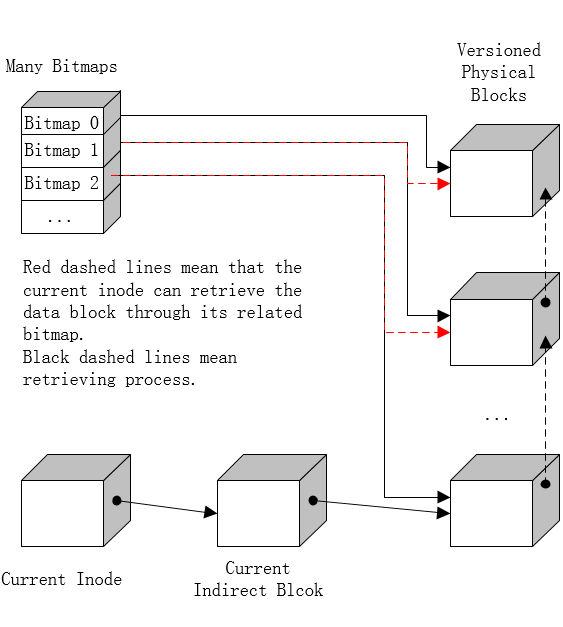
\includegraphics{journal4.png}
\caption{No Inode Duplication Approach}
\end{figure}
There is another promising approach realizing VFS without duplicating the inode. Only an inode is used to represent all versions of a file. There is no timestamp, bitmap, next fields in the inode but it has a pointer which points to a series of blocks containing many bitmaps. each bitmap makes changed blocks according to last version. If users want to get an indexed old version, the system will retrieve the blocks according to each bitmap one version by one version(Figure 5).\\[1em]
It is obviously that this approach saves the space of inode, but it will cost huge time to retrieve an old version. In our consideration, the less retrieving time is more important than the bigger space of metadata. However, if there is optimized mechanism based on this approach which reduce retrieving time, we will then select this one. In conclusion, the duplicated inodes strategy is more suitable to VFS under the current research situation.   
\section*{4~~~~Conclusion}
The above design meets the requirements as outlined in the problem statement mainly by duplicated inodes and COW strategy. The remaining problem is a correct edge check in searching and cache related issue. Perfect unduplicated inode approach and failure tolerance are further research. \\[15em]

Word Count:2500(not include title page)

\end{document}